\documentclass{beamer}

\usepackage{graphicx}
\usepackage[utf8]{inputenc}

\usetheme{Madrid}
\usecolortheme{whale}
\setbeamertemplate{navigation symbols}{}
\title{Automatic Generation of Safety-Critical Test Scenarios for Collision Avoidance of Road Vehicles}
\author{Stefan Huber}
\date{\today}

\begin{document}
\maketitle

\begin{frame}
    \frametitle{How does it work?}
    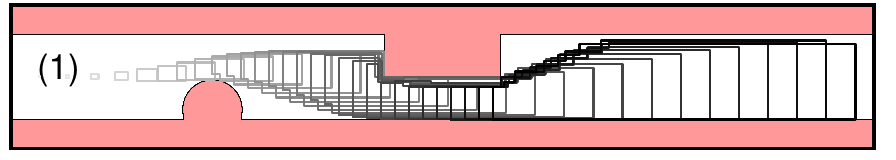
\includegraphics[width=\textwidth]{drivableArea(1).png}
    \pause
    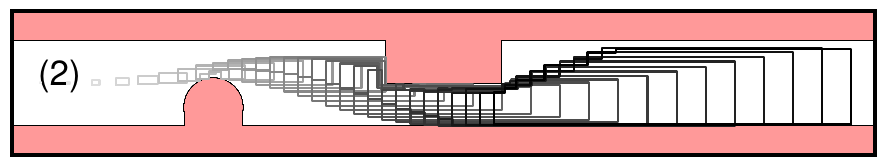
\includegraphics[width=\textwidth]{drivableArea(2).png}
    \pause
    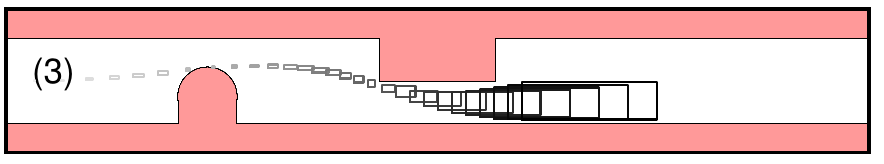
\includegraphics[width=\textwidth]{drivableArea(3).png}
\end{frame}

\begin{frame}
    \frametitle{Questions}
    \begin{itemize}
        \item The approach excludes all area which is occupied at some point in test duration.
            It is not freed if the participant is leaving that area.
            Could there be real benefits?
        \item Safe areas around participants? Maybe based on their speed?
        \item Would you use this approach?
        \item Do you like the paper?
    \end{itemize}
\end{frame}

\end{document}
